\documentclass[12pt]{ctexart} % 使用 ctexart 文档类支持中文

\usepackage{fancyhdr} % 奇特的 header
\usepackage{xcolor} % 更多颜色

\usepackage[utf8]{inputenc} % 支持 UTF8 字符,在 UTF8 engine 中无需此行
\usepackage{xeCJK} % 支持中文排版,已经包含在 ctexart 中
\usepackage{fontspec} % 字体设置
\usepackage{geometry} % 页面布局
\usepackage{titlesec} % 自定义标题样式
\usepackage{setspace} % 设置行距
\usepackage{microtype} % 更多的微调
\usepackage{tabularx} % 表格支持

\usepackage{float} % Add the float package,支持图片位置固定

\usepackage[colorlinks,linkcolor=black,urlcolor=black]{hyperref} % 超链接支持

\usepackage{tocloft} % 自定义目录样式

\usepackage{graphicx} % 图片设置
\graphicspath{ {./images/} }

% 设置页面布局
\geometry{a4paper, margin=1in}

% 设置行距为 1.25 倍
\setstretch{1.25}

% 设置中文字体
\setCJKmainfont{SimSun}[BoldFont={Microsoft YaHei Bold}] % 设置正文为宋体

\setCJKsansfont{Microsoft YaHei}[BoldFont={Microsoft YaHei Bold}] % 标题等无衬线字体为黑体

% 设置英文字体
\setmainfont{Times New Roman}



% 配置页眉和页脚
\pagestyle{fancy}
\fancyhf{}

\renewcommand{\headrulewidth}{0pt}

\setlength{\headheight}{25.60938pt} % Set the headheight to the required value
\addtolength{\topmargin}{-13.60938pt} % Adjust the topmargin to compensate

% 定义颜色
\definecolor{myblue}{RGB}{152, 220, 222} % 蓝色

% 左侧页眉设置, 页码在页眉外侧
\fancyhead[L]{%
  \colorbox{myblue}{%
    \parbox[t]{1cm}{%
      \textcolor{white}{\thepage}%
    }%
  }%
  \hspace{0.5cm}
  设计模式报告
}

% \fancyhead[L]{\leftmark} % 左页显示章节名

% 页眉横线设置
\renewcommand{\headrulewidth}{0.5pt}
\renewcommand{\headrule}{%
  \hbox to\headwidth{%
    \color{black}\leaders\hrule height \headrulewidth\hfill%
  }%
}

% 页脚页数设置
\renewcommand{\footrulewidth}{0pt}
\fancyfoot[C]{\thepage}

% 设置目录样式
\renewcommand{\cftsecfont}{\bfseries} % 目录中章节标题加粗

\titleformat{\section}
  {\normalfont\Large\bfseries} % 移除 \centering
  {\thesection}{1em}{}


% 超链接设置
\hypersetup{
  colorlinks=true,
  linkcolor=black,
  filecolor=magenta,      
  urlcolor=cyan,
}


\begin{document}

\begin{titlepage}
  \centering % 居中对齐
  % \vspace*{1cm} % 从顶部添加一些垂直间距
  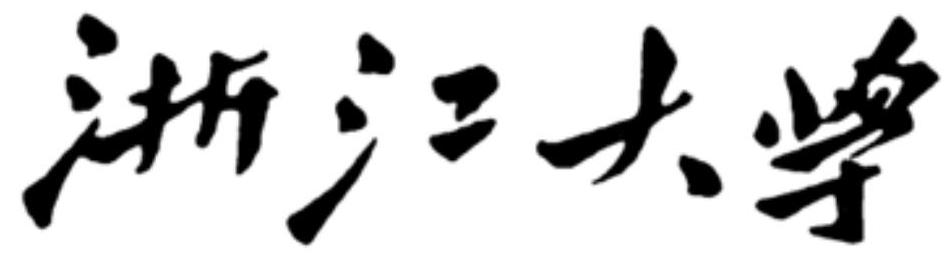
\includegraphics[width=0.6\textwidth]{zjutitle.jpg} % 插入图片
  
  \vspace{2cm} % 添加垂直间距
  
  {\fontsize{36}{48}\selectfont\CJKfontspec{Microsoft YaHei} 设计模式报告} % 标题
  
  \vspace{2cm} % 添加垂直间距
  
  
\includegraphics[width=0.4\textwidth]{zjulogo.jpg} % 插入图片
  
  \vspace{2cm}
  
  {\Huge\CJKfontspec{Microsoft YaHei} 项目主题: \underline{H5游戏分享平台}} % 项目主题 with underline
  
  \vspace{1cm}

  {\Large\CJKfontspec{Microsoft YaHei} 第 1 小组: \underline{XXX}} % 作者
  
  \vspace{1cm} % 添加垂直间距
  
  {\Large\CJKfontspec{Microsoft YaHei} \today} % 日期

\end{titlepage}

\newpage
\tableofcontents % 自动生成目录
\newpage

\section{系统体系分析} % I. 系统体系分析
本项目(H5游戏分享平台)是围绕游戏资源聚合与用户交互为核心的多层架构平台,
主要功能包括游戏上传、用户评论、数据管理等,其核心操作集中于游戏资源的动态管理与用户行为的数据处理。
由于本项目兼具B/S体系架构和典型的数据中心架构的特点,因此我们的设计模式也应与之对应。
同时,由于我们的项目围绕游戏和用户展开,因此游戏的存储结构、不同权限的操作者等都需要进行建模,
这其中其实已经蕴含了许多设计模式。

\section{经典 GOF 设计模式应用} % III. 经典 GOF 设计模式应用
设计模式可以让你避免从零开始设计你的产品,甚至在花费时间和精力后却最终设计出一个不如别人现有产品的东西。
通过使用现有的设计模式,你可以为特定问题获得经过验证的解决方案。随着每种模式的应用,解决方案被整合,要构建的应用程序也就逐渐更接近完整的设计。
使用得当的设计模式,一定会对软件设计有巨大帮助。
因此,我们也对GoF所著的设计模式书籍《设计模式:可复用面向对象软件的基础》进行了学习,并将其中提到的设计模式与当前项目结合起来,具体如下。


\subsection{创建型模式} % 1. 创建型模式
\subsubsection{抽象工厂(Abstract Factory)} 
抽象工厂提供一个创建一系列相关或相互依赖对象的接口,而无需指定它们具体的类。
通过集中决定实例化哪个工厂,它的优点是具有较高的拓展性,当添加新的具体工厂时,无需修改已有代码。
客户端也无需知晓具体实现,只需要调用抽象接口即可。

在网站的UI设计中,我们就可以采用抽象工厂方法,设置抽象工厂类,来进行有关类的实现。
对于UI中的各种元素,如网站整体背景、按钮、图片背景、图标等等,client只需调用UIfactory进行生产,
即可得到不同类型(如明亮或黑暗)的网站元素。这样一来代码更加清晰,同时也实现了各个物品的解耦。
\begin{figure}[H]
  \centering
  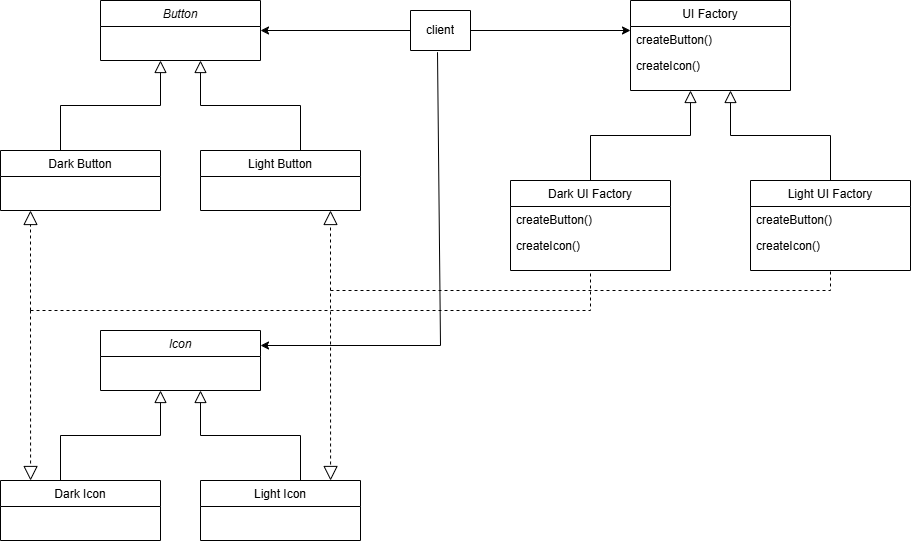
\includegraphics[width=\textwidth]{abs_factory.png}
  \caption{抽象工厂}
\end{figure}

\subsubsection{工厂方法(Factory Method)} 
工厂方法模式在父类中提供一个创建对象的方法,并允许子类决定实例化对象的类型。
这实际上是将类的实例化延迟至子类,使得创建对象的操作更加灵活而不必局限于类的直接创建。

对于浏览本网站的人,它们可能有着不同的身份(如不登录的游客、登录的用户等),因此我们可以单独实现一个类来对它们实现实例化,
而不是通过直接调用这些类自己的构造函数来实例化。如下图所示,client会调用工厂来生成/找到对应的visitor实例。
\begin{figure}[H]
  \centering
  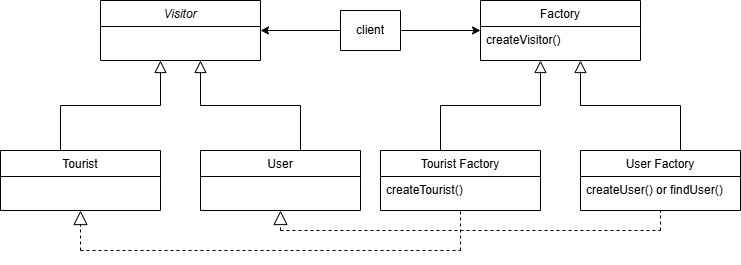
\includegraphics[width=0.8\textwidth]{factory_1.png}
  \caption{身份创建}
\end{figure}

由于在用户新上传游戏或者想要修改老游戏时,网页均会跳转到/upload页面,因此需要设计出一种既能处理新游戏,又能处理老游戏的方法。
事实上,这种复用现有对象的尝试也是工厂方法的一种应用。
通过复用,当处理老游戏时,它会在数据库种搜索对应的游戏id并进行数据展示和修改;而处理新游戏时则会新生成id并存储到数据库中。
\begin{figure}[H]
  \centering
  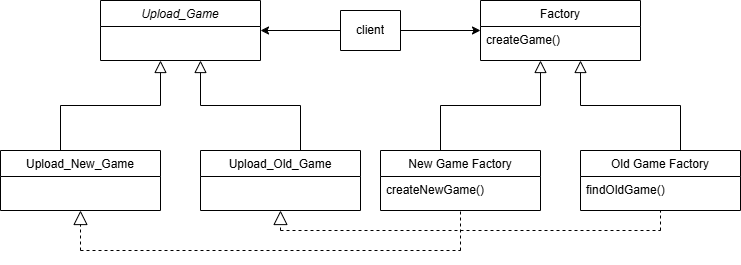
\includegraphics[width=0.8\textwidth]{factory_2.png}
  \caption{上传游戏的处理}
\end{figure}

\subsubsection{生成器(builder)} 
生成器这一设计模式帮助我们分步骤创建复杂对象,并允许使用相同的创建代码和步骤生成不同类型和形式的对象。

假设存在一个复杂对象,它包含许多子对象,因此其嵌套化的初始化导致了构造函数极其复杂。
为了解决这种问题,生成器模式建议将对象构造代码从产品类中抽取出来,并将其放在一个名为生成器的独立对象中。
接着它就会会将对象构造过程划分为一组步骤,并根据特定对象依次调用不同的步骤。

在我们的项目中,游戏对象就是一个明显的复杂对象,它具有较多属性如标题、描述、分类标签、开发者信息等,并且存在可选参数(截图等)。
因此,我们就可以用生成器分离构造过程与对象表示,支持链式调用。
\begin{figure}[H]
  \centering
  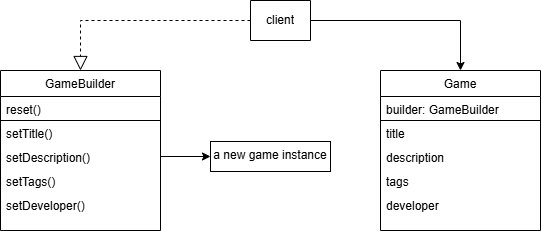
\includegraphics[width=0.8\textwidth]{builder.png}
  \caption{game对象生成}
\end{figure}

\subsubsection{原型(Prototype)} 
原型模式使你能够复制已有对象, 而又无需使代码依赖它们所属的类。
原型模式可以类比细胞的有丝分裂,也和C++代码中的拷贝构造函数有一定的相似性。

在我们的项目中,当我们需要整合某个游戏的不同版本时,我们可以用到原型模式,
并用拷贝构造函数进行实例化。在一个游客通过登录转换为新的正式用户时,
也可以使用原型模式复制一些已经记录的信息。
不过这些用法意义均不大,因此并没有实际应用。

\subsubsection{单件(Singleton)} 
单件模式让你能够保证一个类只有一个实例,并提供一个访问该实例的全局节点。
所有单例的实现都包含以下步骤:
将默认构造函数设为私有, 防止其他对象使用单例类的new运算符;
新建一个静态构建方法作为构造函数。该函数能够调用私有构造函数来创建对象,并将其保存在一个静态成员变量中。
此后所有对于该函数的调用都将返回这一缓存对象。

单件模式同时解决了两个问题,首先,它通过保证一个类只有一个实例,控制某些共享资源(例如数据库或文件)的访问权限。
具体而言,如果你创建了一个对象,同时过一会儿后你决定再创建一个新对象,此时你会获得之前已创建的对象,而不是一个新对象。
像报告中之前提到的各种工厂类其实就可以应用单件模式,因为工厂只需要一个即可。
\begin{figure}[H]
  \centering
  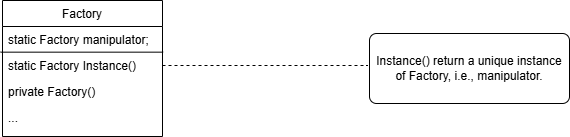
\includegraphics[width=0.8\textwidth]{singleton_1.png}
  \caption{工厂单件}
\end{figure}

其次,单件模式为该实例提供一个全局访问节点。类似于全局变量,它允许在程序的任何地方访问特定对象,并且能够保护该实例不被其他代码覆盖。
在我们的项目中,存储游戏数据以及管理文件的数据库就需要这样的全局访问性,所有的访问都会指向唯一的数据库。
\begin{figure}[H]
  \centering
  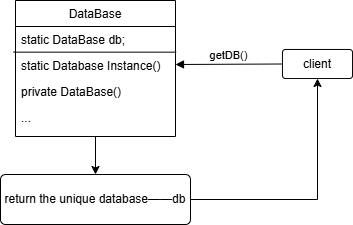
\includegraphics[width=0.8\textwidth]{singleton_2.png}
  \caption{数据库单件}
\end{figure}


\subsection{结构型模式} 
\subsubsection{适配器(Adaptor)} 
适配器模式,它允许接口不兼容的类能够一起工作。
适配器模式通过将一个类的接口转换成客户期望的另一个接口,解决了因接口不兼容而不能一起工作的类的问题。

适配器模式包含以下角色:
目标接口(Target): 客户期望的接口;
适配者(Adaptee): 需要被适配的现有接口;
适配器(Adapter): 将Adaptee接口转换为Target接口;

当代码有多人协作时,我们最初定义的类之间的接口调用可能不再得到实现,从
⽽导致接口相互不兼容,因此我们可以利用适配器模式来实现接口的兼容。
在我们的项目中,当我们对某些数据在不同部分没有严格契合,我们可以用到适配器模
式,并用在少修改代码的情况下引入新的适配器。
\begin{figure}[H]
  \centering
  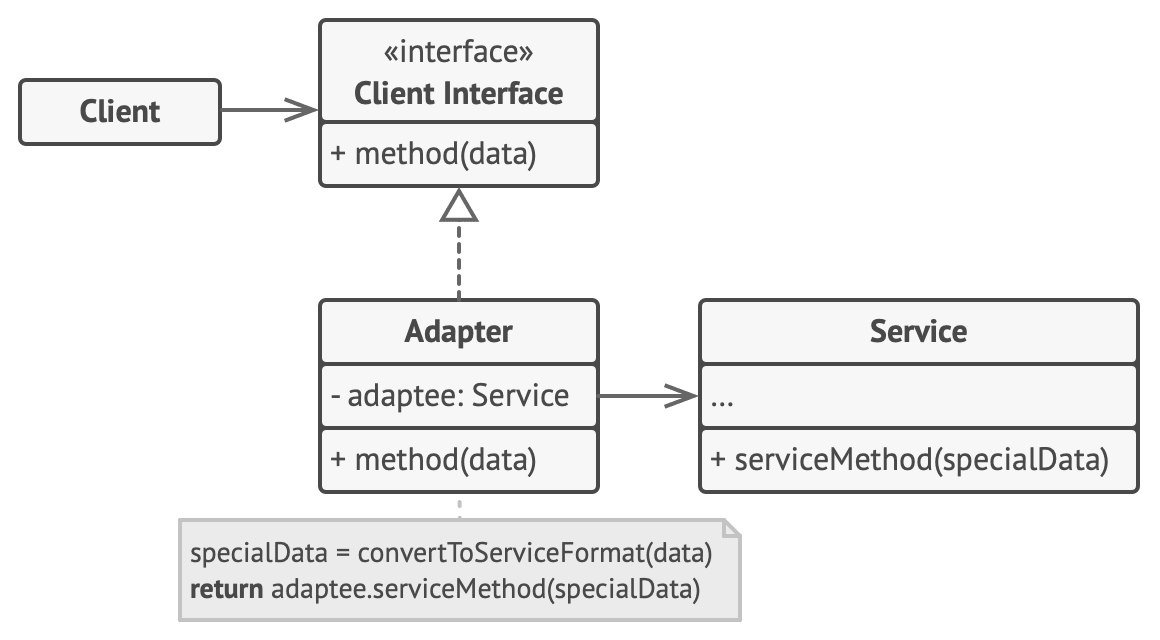
\includegraphics[width=0.7\textwidth]{shipei.png}
  \caption{适配器模式}
\end{figure}

\subsubsection{桥接(Bridge)} 
桥接模式,它将抽象部分与其实现部分分离,使它们可以独立变化。
该模式通过将继承关系改为组合关系来解决多层继承带来的类爆炸问题,
特别适用于一个类存在多个独立变化的维度时。具体来说, 
就是抽取其中一个维度并使之成为独立的类层次, 
这样就可以在初始类中引用这个新层次的对象, 从而使得一个类不必拥有所有的状态和行为。

桥接模式包含以下核心角色:
抽象部分(Abstraction):定义高层控制逻辑,依赖实现部分完成底层操作
扩展抽象(RefinedAbstraction):对抽象部分的扩展
实现部分接口(Implementor):定义实现类的接口
具体实现(ConcreteImplementor):实现Implementor接口的具体类

桥接模式具有两大特点:

解耦抽象与实现:允许抽象和实现独立扩展

提高可扩展性:新增抽象或实现类不影响现有代码

在我们的项目中,我们可以在多端存档同步系统的实现中使用桥接模式
在抽象层:存档数据模型;在实现层:可以有多种同步方式:云存储、本地缓存等
这样可以让我们在存档数据结构稳定情况下,灵活扩展新的同步渠道。
\begin{figure}[H]
  \centering
  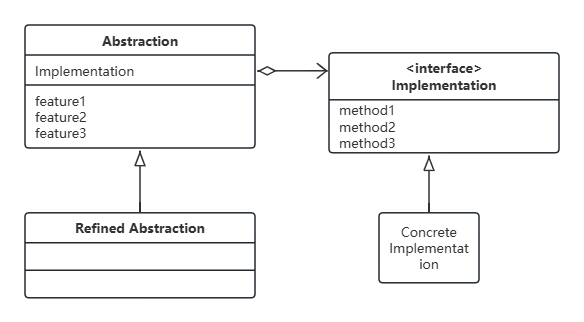
\includegraphics[width=0.7\textwidth]{qiaojie.png}
  \caption{桥接模式}
\end{figure}
\subsubsection{外观(Facade)} 
外观模式,它为复杂的子系统提供了一个简化的接口。
外观模式定义了一个高层接口,使得子系统更容易使用,同时仍然保持对子系统功能的完整访问能力。
其具有:简化接口,解耦,灵活的优点。

外观模式包含以下角色:
外观(Facade): 提供简化的接口,将客户端请求委派给适当的子系统对象;
子系统类(Subsystem classes): 实现子系统的功能,处理外观对象指派的工作;
客户端(Client): 通过外观接口与子系统交互

外观模式适用于以下情况:
需要为复杂的子系统提供一个简单的接口;
客户端与抽象的实现类之间存在很大的依赖性;
需要将子系统分层,使用外观模式定义每个层次的入口点;
我们可以使用外观模式实现
向多个数据分析平台(Google Analytics、腾讯云分析、自有分析系统)上报数据的需求。

\begin{figure}[H]
  \centering
  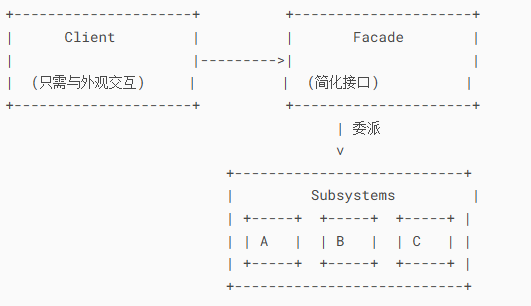
\includegraphics[width=0.7\textwidth]{waiguan.png}
  \caption{外观模式}
\end{figure}

\subsubsection{代理(Proxy)} 
代理模式,它为其他对象提供一种代理以控制对这个对象的访问。
代理对象在客户端和目标对象之间起到中介作用,可以在不改变原始类代码的情况下,
通过引入代理类来增加额外的功能。

代理模式包含以下主要角色:
抽象主题(Subject): 定义真实主题和代理主题的共同接口;
真实主题(Real Subject): 实现真实的业务逻辑;
代理(Proxy): 控制对真实主题的访问,并可以附加额外功能;

代理模式拥有以下优势:
控制访问: 控制客户端对真实对象的访问;
增强功能: 在不修改原始对象的情况下增加额外功能;
解耦: 将客户端与真实对象解耦;
灵活性: 可以根据需要创建不同类型的代理
\begin{figure}[H]
  \centering
  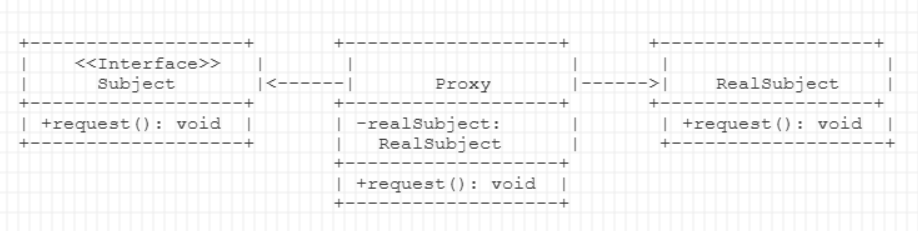
\includegraphics[width=1\textwidth]{daili1.png}
  \caption{代理模式}
\end{figure}

在我们的设计中: H5游戏需要加载大量资源(图片、音频、视频等),直接加载会影响用户体验。
我们可以进行以下的代理模式设计:使用虚拟代理实现资源的延迟加载和按需加载;
加载过程中显示占位图或加载动画;对加载失败资源进行智能替换或重试。
\begin{figure}[H]
  \centering
  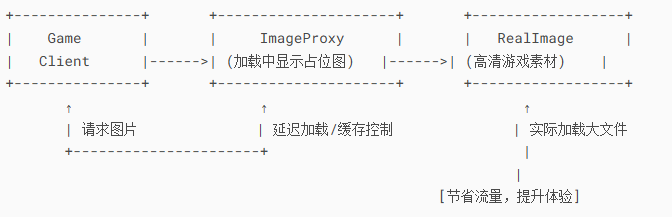
\includegraphics[width=1\textwidth]{daili2.png}
  \caption{应用示例}
\end{figure}
\subsection{行为模式}  
\subsubsection{迭代器(Iterator)} 
迭代器模式,它提供一种顺序访问聚合对象(如集合、列表、树等)中元素的方法,而无需暴露其底层表示。
其核心思想是将遍历逻辑与数据结构分离,使客户端可以统一处理不同类型的集合。
除实现自身算法外, 迭代器还封装了遍历操作的所有细节, 例如当前位置和末尾剩余元素的数量。 
因此, 多个迭代器可以在相互独立的情况下同时访问集合。

所有迭代器必须实现相同的接口。 这样一来, 只要有合适的迭代器, 客户端代码就能兼容任何类型的集合或遍历算法。 
如果你需要采用特殊方式来遍历集合, 只需创建一个新的迭代器类即可, 无需对集合或客户端进行修改。

在我们的设计中,通过使用迭代器模式,我们能较好地实现动态加载游戏资源(图片、音频等游戏数据),
避免一次性加载导致卡顿。同时可以相应实现按需加载资源,优化内存使用;支持优先级遍历(先加载关键资源)
\begin{figure}[H]
  \centering
  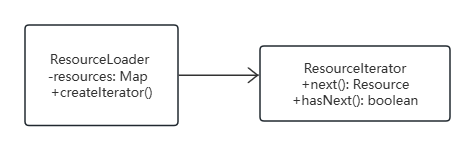
\includegraphics[width=1\textwidth]{diedai.png}
  \caption{迭代器模式示例}
\end{figure}
\subsubsection{备忘录(Memento)} 
备忘录模式,它允许在不破坏对象封装性的前提下,捕获并外部化对象的内部状态,以便后续可以恢复到这个状态。
其实现主要分为三个部分:Originator:需要保存状态的对象,提供创建/恢复备忘录的方法
Memento:存储Originator内部状态的对象(通常不可修改)
CareTaker:管理备忘录历史记录,但不直接操作备忘录内容

备忘录模式将创建状态快照 (Snapshot) 的工作委派给实际状态的拥有者原发器 (Originator) 对象。 
这样其他对象就不再需要从 “外部” 复制编辑器状态了, 编辑器类拥有其状态的完全访问权, 因此可以自行生成快照。
模式建议将对象状态的副本存储在一个名为备忘录 (Memento) 的特殊对象中。 
除了创建备忘录的对象外, 任何对象都不能访问备忘录的内容。 
其他对象必须使用受限接口与备忘录进行交互, 它们可以获取快照的元数据 (
创建时间和操作名称等), 但不能获取快照中原始对象的状态。

备忘录模式可以帮助我们实现玩家编辑的较为复杂的内容(如文字+截图)临时保存的功能,
更进一步的,可以实现玩家在不同设备上回复游戏进度,以及退回操作,即回档的功能。
\begin{figure}[H]
  \centering
  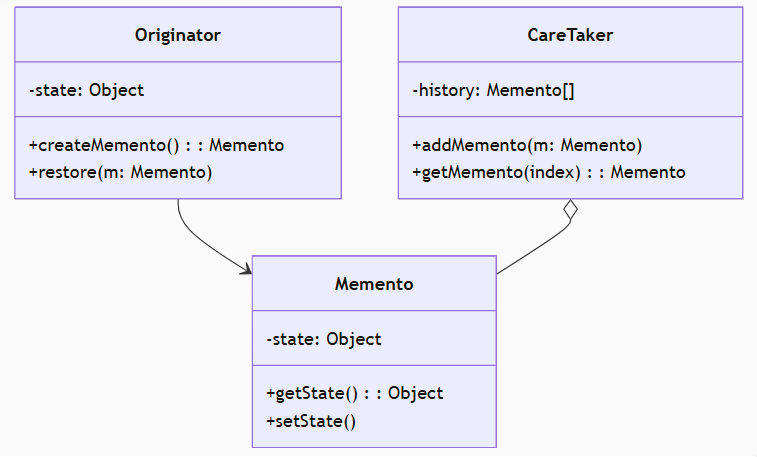
\includegraphics[width=1\textwidth]{beiwang.png}
  \caption{备忘录模式示例}
\end{figure}

\subsubsection{观察者(Observer)}
观察者模式它定义了一种一对多的依赖关系,
当一个对象(Subject)的状态发生改变时,所有依赖于它的对象(Observers)都会自动收到通知并更新。

拥有一些值得关注的状态的对象通常被称为目标, 由于它要将自身的状态改变通知给其他对象, 
我们也将其称为发布者 (publisher)。 所有希望关注发布者状态变化的其他对象被称为订阅者 (subscribers)
在实现中,所有订阅者都应该实现同样的接口, 发布者仅通过该接口与订阅者交互。 
接口中必须声明通知方法及其参数, 这样发布者在发出通知时还能传递一些上下文数据。
在我们的项⽬中,观察者模式可以应⽤在当游戏创作者通知收藏了自己游戏的用户(如游戏更新通知)
以及管理员像某些用户发送通知的功能上

\begin{figure}[H]
  \centering
  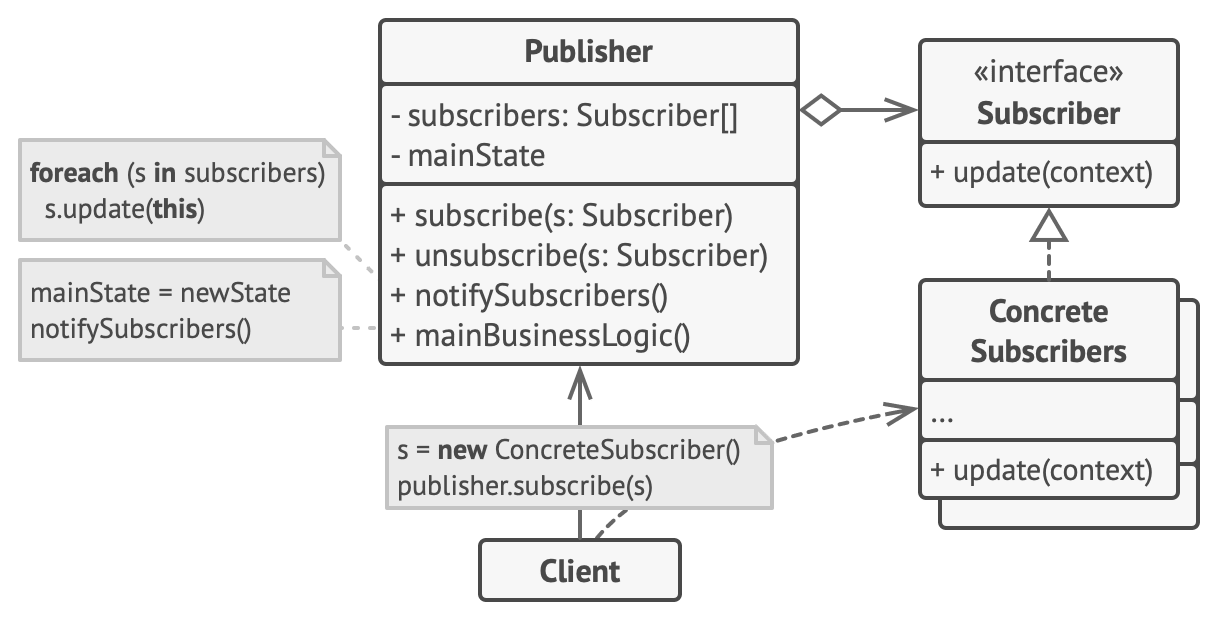
\includegraphics[width=1\textwidth]{guancha.png}
  \caption{观察者模式}
\end{figure}

\subsubsection{状态(State)} 
状态模式 能让你在一个对象的内部状态变化时改变其行为,使其看上去就像改变了自身所属的类一样。

状态模式与有限状态机 的概念紧密相关。
其主要思想是程序在任意时刻仅可处于几种有限的状态中。 在任何一个特定状态中, 程序的行为都不相同, 
且可瞬间从一个状态切换到另一个状态。不过,根据当前状态,
程序可能会切换到另外一种状态, 也可能会保持当前状态不变。 
这些数量有限且预先定义的状态切换规则被称为转移。
我认为其设计的核心功能有:
消除条件分支:用多态代替状态判断语句
状态封装:每个状态都是一个独立的类
动态切换:运行时自由切换状态对象

在我们的设计中,游戏玩家可能处于游客、已登录、封禁等不同状态,各状态下的功能权限不同
以及平台中的一些资源加载需处理初始化、加载中、就绪、失败等状态。
我们可以采用状态模式的设计来实现这些设计。

\begin{figure}[H]
  \centering
  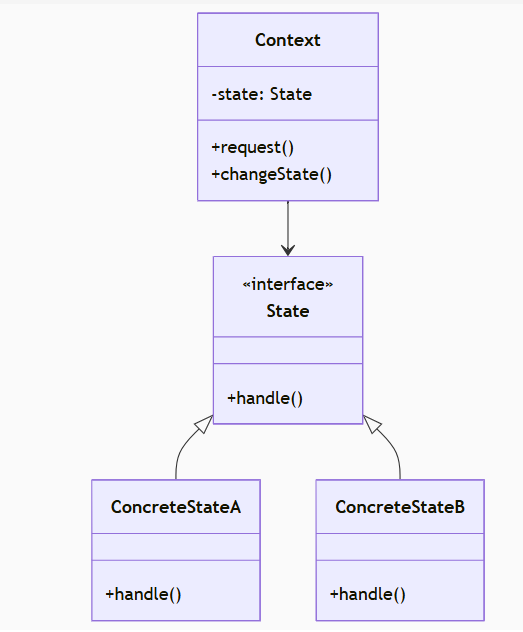
\includegraphics[width=1\textwidth]{zhuangtai.png}
  \caption{状态模式}
\end{figure}

\subsubsection{策略(Strategy)} 
策略模式中,它能让你定义一系列算法, 
并将每种算法分别放入独立的类中, 以使算法的对象能够相互替换,让算法的变化独立于使用它的客户端
同时可以让我们在运行时切换,动态选择最佳策略。

我们需要找出负责用许多不同方式完成特定任务的类, 然后将其中的算法抽取到一组被称为策略的独立类中。
名为上下文的原始类必须包含一个成员变量来存储对于每种策略的引用。 上下文并不执行任务, 
而是将工作委派给已连接的策略对象。

使用策略模式,我们可以对不同的用户设置符合他们的服务,如根据设备性能/屏幕尺寸自动调整UI布局
以提升不同设备用户的体验一致性,不同网络条件下的通信方案。

\begin{figure}[H]
  \centering
  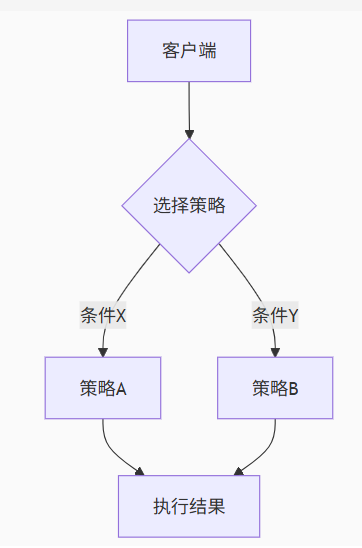
\includegraphics[width=0.8\textwidth]{celv.png}
  \caption{策略模式}
\end{figure}

\subsubsection{模板方法(Template Method)} 
模板方法模式它在一个方法中定义了一个算法的骨架,而将一些步骤延迟到子类中实现。
模板方法使得子类可以在不改变算法结构的情况下,重新定义算法中的某些步骤。
模板方法模式的设计可以实现标准化流程:固定算法执行顺序;
灵活扩展:子类可定制关键步骤;
避免重复:公共逻辑提升至父类

数据的上报需经过(收集→加密→压缩→传输),但加密/压缩方式因数据类型而异。
对此我们可以采用模板方法模式:

[数据上报模板]

├─ 1. 收集原始数据 (固定实现)

├─ 2. 执行数据加密 (抽象步骤)

├─ 3. 进行内容压缩 (抽象步骤)

└─ 4. 网络传输 (固定实现)

\begin{figure}[H]
  \centering
  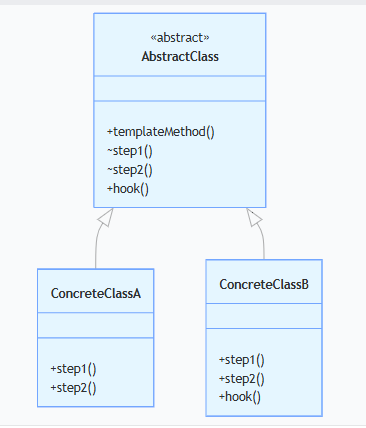
\includegraphics[width=0.8\textwidth]{moshi.png}
  \caption{模板方法模式}
\end{figure}

\section{参考文献} % IV. 参考文献
1.《设计模式:可复用面向对象软件的基础》

2.设计模式网站:https://refactoringguru.cn/

\end{document}